\section{Experiments}
This section focuses on the results gotten from the conducted experiments. These will first briefly be presented in section \ref{results}. After that, section \ref{exp:int} will discuss them in more detail, and see how they compare to earlier studies, etc.

\subsection{Results} \label{results}
Results are presented in the form of tables and line plots. The former of these reports final testing performance, whereas the latter mostly visualizes validation accuracy during training.

To give a more precise description: tables show average testing performance over the 5 trials per experiment, with standard deviation ($s$) as a subscript. Besides accuracy, also balanced accuracy is reported. This measure is defined as the average recall over all classes, such that it penalizes errors on less occurring classes more than plain accuracy would. Lastly, green shaded cells mark best performance, while yellow and red mark second best and worst performance, respectively.

For line plots, shaded regions correspond to the \textit{standard error of the mean} ($\pm s \div \sqrt{N}$, where $N=5$). In cases where they show average validation accuracy, plots end when an early stop occurred for the first of 5 trials. To easily distinguish VTs from CNNs, VTs are plotted with continuous lines, and CNNs with dashed ones.

\subsubsection{Off-the-shelf learning} \label{results:ots}

\begin{figure*}[tb]
    \centering
    \def\svgwidth{\textwidth}
    \input{img/ots_mean_accuracy.pdf_tex}
    \caption{Average validation accuracy when training with an off-the-shelf learning scheme. It can be observed that the \texttt{Swin} VT achieves the highest performance overall, but that the \texttt{ConvNext} CNN is a close second. More general, VTs perform on par with CNNs, if not slightly better.}
    \label{results:img:ots}
\end{figure*}

\begin{table*}[tb]
\centering
\resizebox{\textwidth}{!}{%
\begin{tabular}{lllllll}
\hline
\textbf{Model} & \textbf{Type} &  & \textbf{Material} & & \textbf{Artist} & \\
& \textbf{Accuracy} & \textbf{Bal. accuracy} & \textbf{Accuracy} & \textbf{Bal. accuracy} & \textbf{Accuracy} & \textbf{Bal. accuracy} \\ \hline
\textbf{vit\_b\_16} & 86.06\% $_{\pm 1.06\%}$ & 84.13\% $_{\pm 1.57\%}$ & 81.78\% $_{\pm 0.48\%}$ & 67.38\% $_{\pm 1.37\%}$ & 84.89\% $_{\pm 0.46\%}$ & 81.42\% $_{\pm 0.42\%}$  \\
\textbf{swin\_b} & \cellcolor{bestcol}89.43\% $_{\pm 0.93\%}$ & \cellcolor{bestcol}87.47\% $_{\pm 1.02\%}$ & \cellcolor{bestcol}85.87\% $_{\pm 0.35\%}$ & \cellcolor{bestcol}71.19\% $_{\pm 1.60\%}$ & \cellcolor{bestcol}90.40\% $_{\pm 0.65\%}$ & \cellcolor{bestcol}88.64\% $_{\pm 0.78\%}$  \\
\textbf{beit\_b\_16} & \cellcolor{worstcol}82.26\% $_{\pm 0.72\%}$ & \cellcolor{worstcol}77.75\% $_{\pm 0.27\%}$ & 76.87\% $_{\pm 0.96\%}$ & 60.16\% $_{\pm 1.56\%}$ & 79.70\% $_{\pm 0.69\%}$ & 75.35\% $_{\pm 1.09\%}$  \\
\textbf{deit\_b\_16} & 88.18\% $_{\pm 0.66\%}$ & 85.36\% $_{\pm 0.54\%}$ & 82.80\% $_{\pm 1.12\%}$ & 66.46\% $_{\pm 1.03\%}$ & 88.13\% $_{\pm 0.76\%}$ & 85.62\% $_{\pm 0.87\%}$  \\\hdashline
\textbf{vgg19} & 83.93\% $_{\pm 0.72\%}$ & 83.35\% $_{\pm 0.81\%}$ & 76.87\% $_{\pm 0.44\%}$ & 61.39\% $_{\pm 1.47\%}$ & 82.01\% $_{\pm 0.66\%}$ & 78.10\% $_{\pm 0.77\%}$  \\
\textbf{resnet50} & 85.51\% $_{\pm 0.64\%}$ & 82.33\% $_{\pm 1.85\%}$ & 80.99\% $_{\pm 0.82\%}$ & 65.51\% $_{\pm 0.93\%}$ & 87.71\% $_{\pm 1.06\%}$ & 85.12\% $_{\pm 1.34\%}$  \\
\textbf{eff. netv2\_m} & 83.41\% $_{\pm 0.76\%}$ & 82.05\% $_{\pm 1.25\%}$  & \cellcolor{worstcol}75.96\% $_{\pm 1.24\%}$ & \cellcolor{worstcol}59.15\% $_{\pm 1.24\%}$ & \cellcolor{worstcol}78.62\% $_{\pm 1.07\%}$ & \cellcolor{worstcol}73.92\% $_{\pm 0.96\%}$  \\
\textbf{convnext\_b} & \cellcolor{secondbestcol}89.19\% $_{\pm 0.64\%}$ & \cellcolor{secondbestcol}86.95\% $_{\pm 1.38\%}$ & \cellcolor{secondbestcol}84.14\% $_{\pm 0.92\%}$ & \cellcolor{secondbestcol}69.10\% $_{\pm 1.05\%}$ & \cellcolor{secondbestcol}90.13\% $_{\pm 0.94\%}$ & \cellcolor{secondbestcol}87.84\% $_{\pm 1.07\%}$  \\\hline
\end{tabular}
}
\caption{Testing performance after off-the-shelf learning. Results are similar to validation accuracy shown in Figure \ref{results:img:ots}, with \texttt{Swin} and \texttt{ConvNext} showing the respective best and second best performance in all cases.}
\label{results:tab:ots}
\end{table*}

Table \ref{results:tab:ots} shows the testing performance of OTS-trained models on the 3 classification tasks, while Figure \ref{results:img:ots} shows corresponding validation accuracies. Performance on the testing set is comparable among all tasks in terms of rankings. Other observations are consistent as well, such as \texttt{ConvNext} taking the most epochs to converge.

VTs perform very much on par with CNNs, if not slightly better. The best-performing model, for instance, is the \texttt{Swin} VT, which shows the highest testing performance without exception. Moreover, all VTs except \texttt{BeiT} are positioned relatively high in the rankings. This is also reflected in their combined average accuracies being higher than those of CNNs. To give \textit{Type classification} as an example: here VTs as a group achieve an 86.5\% mean accuracy, while this is 85.5\% for CNNs.

Finally, when comparing the 3 classification tasks to one another, it can be observed that the highest overall accuracies are achieved for \textit{Artist classification}, and the lowest ones for \textit{Material classification}. For balanced accuracy, the differences are more extreme, as this measure also falls behind plain accuracy the most for \textit{Material classification}, and the least for \textit{Artist classification}.

% Results favorable for VTs:
%    - Best performing model = VT (SWIN)
%    - 3 of 4 VTs on top ?
%    - Avg of all VTs better than avg CNNs

% Talk about differences between experiments
% Talk about balanced accuracy?

\subsubsection{Fine-tuning} \label{results:ft}

\begin{figure*}[tb]
    \centering
    \def\svgwidth{\textwidth}
    \input{img/ft_mean_accuracy.pdf_tex}
    \caption{Average validation accuracy when fine-tuning models on the target task. Overall, performance is higher compared to off-the-shelf learning in Figure \ref{results:img:ots}, while the differences between models are also smaller here. The \texttt{Swin} VT and \texttt{ConvNext} CNN remain the best performing models, while in general, results are less favorable for VTs than they were after off-the-shelf learning.}
    \label{results:img:ft}
\end{figure*}

\begin{table*}[tb]
\centering
\resizebox{\textwidth}{!}{%
\begin{tabular}{lllllll}
\hline
\textbf{Model} & \textbf{Type} &  & \textbf{Material} & & \textbf{Artist} & \\
& \textbf{Accuracy} & \textbf{Bal. accuracy} & \textbf{Accuracy} & \textbf{Bal. accuracy} & \textbf{Accuracy} & \textbf{Bal. accuracy} \\ \hline
\textbf{vit\_b\_16} & \cellcolor{worstcol}90.11\% $_{\pm 0.35\%}$ & 87.40\% $_{\pm 0.29\%}$ & 87.42\% $_{\pm 0.45\%}$ & 73.46\% $_{\pm 1.44\%}$ & 92.05\% $_{\pm 0.44\%}$ & 89.77\% $_{\pm 0.38\%}$  \\
\textbf{swin\_b} & \cellcolor{bestcol}92.17\% $_{\pm 0.98\%}$ & \cellcolor{secondbestcol}89.71\% $_{\pm 1.03\%}$ & \cellcolor{bestcol}89.35\% $_{\pm 0.68\%}$ & 77.16\% $_{\pm 2.98\%}$ & \cellcolor{bestcol}95.05\% $_{\pm 0.47\%}$ & \cellcolor{bestcol}93.94\% $_{\pm 0.81\%}$  \\
\textbf{beit\_b\_16} & 90.81\% $_{\pm 0.41\%}$ & 87.95\% $_{\pm 0.69\%}$ & \cellcolor{worstcol}85.74\% $_{\pm 0.37\%}$ & \cellcolor{worstcol}72.12\% $_{\pm 1.38\%}$ & \cellcolor{worstcol}91.27\% $_{\pm 1.13\%}$ & \cellcolor{worstcol}88.83\% $_{\pm 1.63\%}$  \\
\textbf{deit\_b\_16} & 91.78\% $_{\pm 0.64\%}$ & 89.22\% $_{\pm 0.90\%}$ & 87.85\% $_{\pm 1.12\%}$ & 74.42\% $_{\pm 1.99\%}$ & 93.37\% $_{\pm 1.15\%}$ & 91.67\% $_{\pm 1.55\%}$  \\\hdashline
\textbf{vgg19} & 90.54\% $_{\pm 0.37\%}$ & \cellcolor{worstcol}87.05\% $_{\pm 1.03\%}$ & 85.74\% $_{\pm 1.40\%}$ & 72.43\% $_{\pm 3.03\%}$ & 92.20\% $_{\pm 0.49\%}$ & 90.18\% $_{\pm 0.72\%}$  \\
\textbf{resnet50} & 91.78\% $_{\pm 0.44\%}$ & 88.24\% $_{\pm 0.59\%}$ & 88.69\% $_{\pm 0.99\%}$ & \cellcolor{secondbestcol}77.97\% $_{\pm 2.25\%}$ & \cellcolor{secondbestcol}94.72\% $_{\pm 0.74\%}$ & \cellcolor{secondbestcol}93.41\% $_{\pm 1.05\%}$  \\
\textbf{eff. netv2\_m} & 90.87\% $_{\pm 0.67\%}$ & 88.34\% $_{\pm 1.37\%}$ & 87.55\% $_{\pm 1.15\%}$ & 75.31\% $_{\pm 1.60\%}$ & 92.65\% $_{\pm 0.54\%}$ & 90.84\% $_{\pm 0.51\%}$  \\
\textbf{convnext\_b} & \cellcolor{secondbestcol}92.15\% $_{\pm 0.40\%}$ & \cellcolor{bestcol}89.82\% $_{\pm 1.18\%}$ & \cellcolor{secondbestcol}88.79\% $_{\pm 1.07\%}$ & \cellcolor{bestcol}78.40\% $_{\pm 1.26\%}$ & 94.60\% $_{\pm 0.54\%}$ & 93.13\% $_{\pm 0.61\%}$  \\\hline
\end{tabular}
}
\caption{Testing performance after fine-tuning. Results are again similar to validation accuracy in Figure \ref{results:img:ft}. Compared to Table \ref{results:tab:ots}, it is striking that the \texttt{ConvNext} CNN now often takes the lead with respect to balanced accuracy, and that the \texttt{ResNet50} CNN often takes second place.}
\label{results:tab:ft}
\end{table*}

Once again, Table \ref{results:tab:ft} shows testing performance, while Figure \ref{results:img:ft} shows validation accuracies.

Results are less favorable for VTs than they were after OTS learning in section \ref{results:ots}. At the same time, it can still be said that VTs perform on par with CNNs. The \texttt{Swin} VT shows the best overall testing accuracy here as well, but the \texttt{ConvNext} CNN is not far behind, and outperforms \texttt{Swin} in terms of balanced accuracy. Also noteworthy is the \texttt{ResNet50} CNN, which is ranked higher here than it was for OTS learning, and now shows the second best testing performance for \textit{Artist classification}.

VTs and CNNs grouped are much more evenly matched. To again take \textit{Type classification} as an example: the mean testing accuracy of all VTs combined is 91.2\% on this task, while it is 91.3\% for CNNs. Recall that section \ref{results:ots} reported a difference of 1\% in favor of VTs here, with an accuracy of 86.5\% for VTs, and 85.5\% for CNNs.

More generally, it can be observed that FT leads to substantially better performance than OTS learning, and that models are now much closer together. The difference between the highest and lowest testing accuracy, for example, is at most 3.8\% after FT, while it was between 7.2\% and 11.8\% after OTS learning. In addition, the worst testing accuracy after FT is most often still higher than the best accuracy after OTS learning. The only exception is \textit{Material classification}, where the worst FT model (\texttt{BeiT}) has an accuracy of 85.74\%, and the best OTS one (\texttt{Swin}) has 85.87\%.

Lastly, note that the highest overall performances are again achieved on the \textit{Artist classification} task, while the lowest ones are reported for \textit{Material classification}. The difference between plain and balanced accuracy is also again the largest for \textit{Material classification}, and lowest for \textit{Artist classification}.

% Results less favourable compared to OTS
%    - Swin still best, tho more debatable
%    - ConvNext catching up
%    - ResNet interesting
%    - As groups: no differences anymore really

% Overall:
%    - higher
%    - closer together
%    - for all but one worst FT is better than best OTS
%    - same observations when comparing tasks to one another

\subsubsection{Scaling}

\begin{figure*}[tb]
    \centering
    \def\svgwidth{\textwidth}
    \input{img/scaling_accuracy.pdf_tex}
    \caption{Testing accuracy as datasets gradually become smaller. The x-axes show a logarithmic scale, with the smallest value being roughly 10\% the size of the largest one. Observations done in sections \ref{results:ots} and \ref{results:ft} appear to hold up well as the training set is shrunk.}
    \label{results:img:scale}
\end{figure*}

Figure \ref{results:img:scale} shows how testing accuracy decreases when smaller portions of the full dataset are taken (see section \ref{methods:dataset}). The x-axes show a logarithmic scale, where each successive value is roughly 56\% the size of its predecessor.

For both OTS learning as FT, findings done in sections \ref{results:ots} and \ref{results:ft} seem to hold up as dataset sizes are shrunk. It is not true, for example, that at some point CNNs start to outperform VTs. In addition, \texttt{Swin} and \texttt{ConvNext} remain some of the best-performing models throughout. 

Lastly, when going from largest to smallest dataset, the mean accuracy of all models taken together drops with 9.1\% for OTS learning. For FT this is 9.2\%, which is very similar. This, then, does not suggest that at some point OTS learning becomes preferred due to overfitting problems for FT.


\subsection{Discussion} \label{exp:int} % TODO maybe change to Interpretation instead
While most results have now been presented, it is still important to discuss them in more detail, as this leads to a more complete interpretation. This subsection attempts to provide such a discussion, by answering questions one might have at this moment. It will first address some of the aforementioned experiments individually, but will conclude with more general remarks. Topics will include: comparisons with earlier studies, potential shortcomings, and hypotheses that might explain certain observations.

\subsubsection{Off-the-shelf learning}

\paragraph{How do these results compare to related studies?}
Of all related work mentioned in section \ref{related_work}, \citeauthor{zhou2021convnets} (\citeyear{zhou2021convnets}) was the only one that examined VTs' OTS learning properties. It reported the best OTS learning performance for the \texttt{Swin} VT, which is much in line with the results in Table \ref{results:tab:ots}.

Besides \texttt{Swin}, \citeauthor{zhou2021convnets} also included \texttt{ViT} and \texttt{ResNet101} in its comparisons (among others), and consistently found that \texttt{ResNet101} outperformed \texttt{ViT}. The current study, on the other hand, uses \texttt{ResNet50}, which performs worse than \texttt{ViT} on all tasks except \textit{Artist classification}. Running the same experiments with \texttt{ResNet101} does, however, lead to similar findings as \citeauthor{zhou2021convnets}. On \textit{Type classification}, for example, it achieves a mean testing accuracy of  $86.21\% (\pm 0.70\%)$, which is indeed slightly higher than \texttt{ViT}'s 86.06\% shown in Table \ref{results:tab:ots}. Mind that these differences are slight compared to the 89.43\% accuracy achieved by \texttt{Swin} here, so replacing \texttt{ResNet50} with \texttt{ResNet101} would not have affected the overall observations that much.

Finally, because \texttt{VGG19} was specifically selected for its good OTS performance in \citeauthor{sabatelli2018deep} (\citeyear{sabatelli2018deep}), it is interesting that this model is outperformed by \texttt{ResNet50} (which that paper also included) in Table \ref{results:tab:ots}. \texttt{VGG19} is the largest model of all, so this discrepancy could be an indication that the smaller datasets used in the current study are too small for \texttt{VGG19}. Additionally, it might also be attributable to the smaller number of classes used here: \texttt{VGG19} has the largest final layer, containing 4096 inputs. While in \citeauthor{sabatelli2018deep} this might have provided the expressive power needed to differentiate between a few hundred classes after just OTS learning, here it likely causes overfitting before good convergence is reached.

\paragraph{Why do VTs perform so well here?}

\begin{figure*}[tb]
    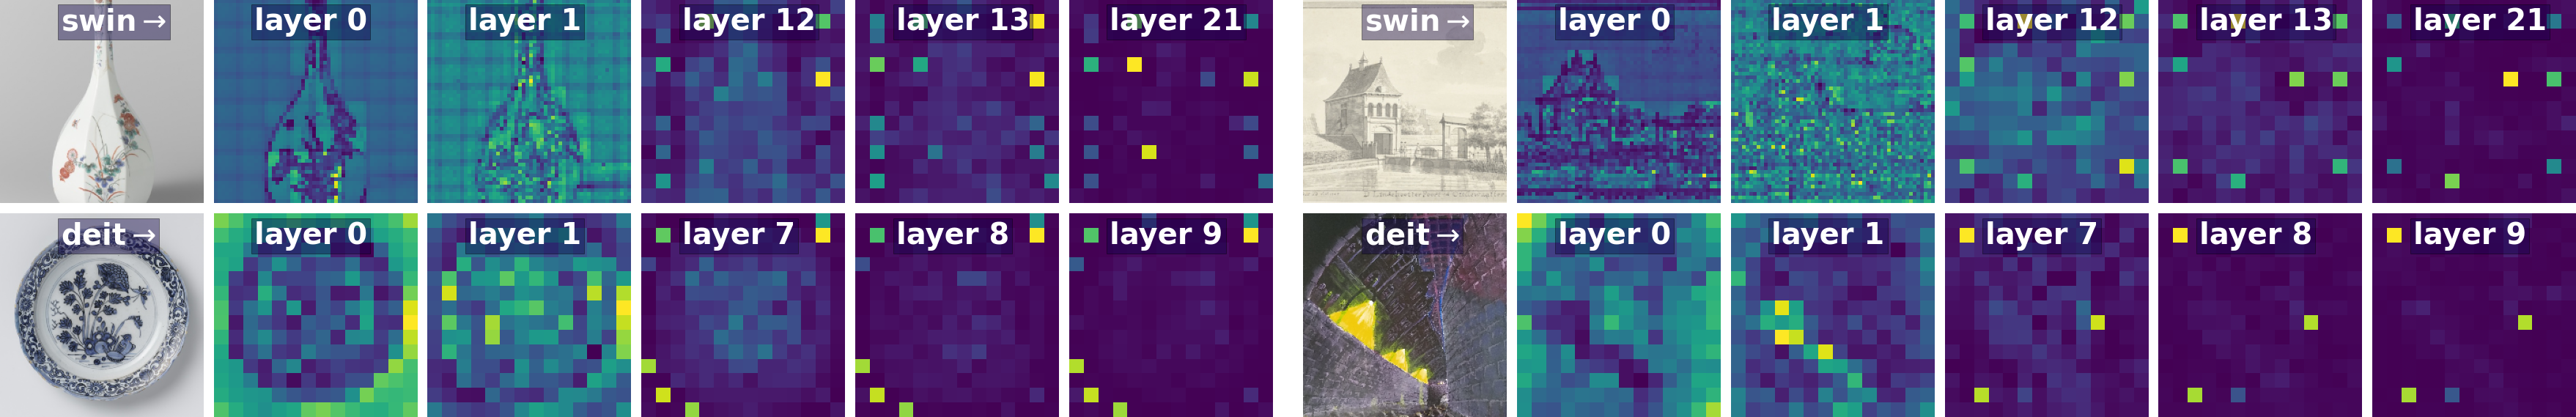
\includegraphics[width=\textwidth]{img/layers.png}
    \caption{Attention layers of successively deeper transformer blocks. One can recognize the input image in earlier layers, while for later ones, activation seems sporadic. For \texttt{DeiT}, attention with respect to the class-token is plotted. \texttt{Swin}, on the other hand, does not have a class-token, so average overall attention is used instead. In addition, the window-shifting operations of this architecture are counteracted.}
    \label{results:img:layers}
\end{figure*}

While results are in line with previous studies, it was still surprising to see that VTs showed such good OTS learning performance in section \ref{results:ots}. It suggests that these transformer-based architectures are able to give a very complete, high-level encoding of the input image. For CNNs this is commonly thought to be true, as they are often described as hierarchical feature extractors that build successively higher-level feature maps from lower-level ones (see section \ref{intro:cnns}). If the same is true for VTs, is not well understood at this moment. Or at least to the best of the author's knowledge, that is.

A hint of an answer can, however, be found when plotting activation of successively deeper attention layers, as is done in Figure \ref{results:img:layers}. While earlier layers retain much spatial information, later ones show more sporadic activation patterns. This is what one might expect from a hierarchical feature extractor: the random pixels lighting up might, for example, correspond to specific, high-level properties of the input. Nevertheless, it should be emphasized that no strong conclusions should be drawn from these images, and that more research with respect to explainability is desired.
% Also mention that this was unexpected (but in line with blabla);
% Feature extractor/hierarchical representation building
% Layers img.
% Maybe mention that image specific inductive bias isn't a problem for swin? TODO somewhere else!

\subsubsection{Fine-tuning} \label{exp:int:ft}

\paragraph{How do these results compare to related studies?}
That the \texttt{Swin} VT performs well after FT, is again consistent with \citeauthor{zhou2021convnets} (\citeyear{zhou2021convnets}). In that paper, however, \texttt{ViT} outperforms the \texttt{ResNet101} and \texttt{ResNet152} CNNs. This differs from the results in Table \ref{results:tab:ft}, where \texttt{ViT} does not perform well overall, and even shows the worst testing accuracy on \textit{Type classification}, with 90.11\%. \texttt{ResNet50} achieves 91.78\% accuracy here, and testing the same \texttt{ResNet101} and \texttt{ResNet152} versions that \citeauthor{zhou2021convnets} used does not change much, as this leads to 91.96\% ($\pm$ 0.59\%) and 91.94\% ($\pm$ 0.25) accuracy, respectively.

Results are also less favorable for VTs compared to \citeauthor{matsoukas2021time} (\citeyear{matsoukas2021time}). In that paper, the `tiny' version of \texttt{DeiT} outperforms \texttt{ResNet50}, while in Table \ref{results:tab:ft} this same \texttt{ResNet50} performs slightly better than the `base' version of \texttt{DeiT}. Going `tiny' also does not help: on \textit{Type classification}, for instance, `tiny' \texttt{DeiT} gets 90.44\% ($\pm$ 0.93\%), which is even worse than `base' \texttt{DeiT}'s 91.78\% in Table \ref{results:tab:ots}.

These slight performance differences could be attributable to the different datasets used. In that case, it seems, VTs have certain strengths that those other datasets take more advantage of. Alternatively, it could be that hyperparameters and regularisation still leave room for improvement. The reason for thinking this, is that preliminary experiments suggested that VTs benefit more from regularisation than CNNs do.

Finally, it was observed that \texttt{ResNet50} appears to flourish with FT, sometimes even beating \texttt{Conv\-Next} in the rankings. This is consistent with \citeauthor{sabatelli2018deep} (\citeyear{sabatelli2018deep}), where it was the best FT model overall.

\paragraph{Why are results less favorable for VTs after FT than after OTS learning?}

\begin{figure*}[tb]
    \centering
    \begin{subfigure}{0.49\textwidth}
    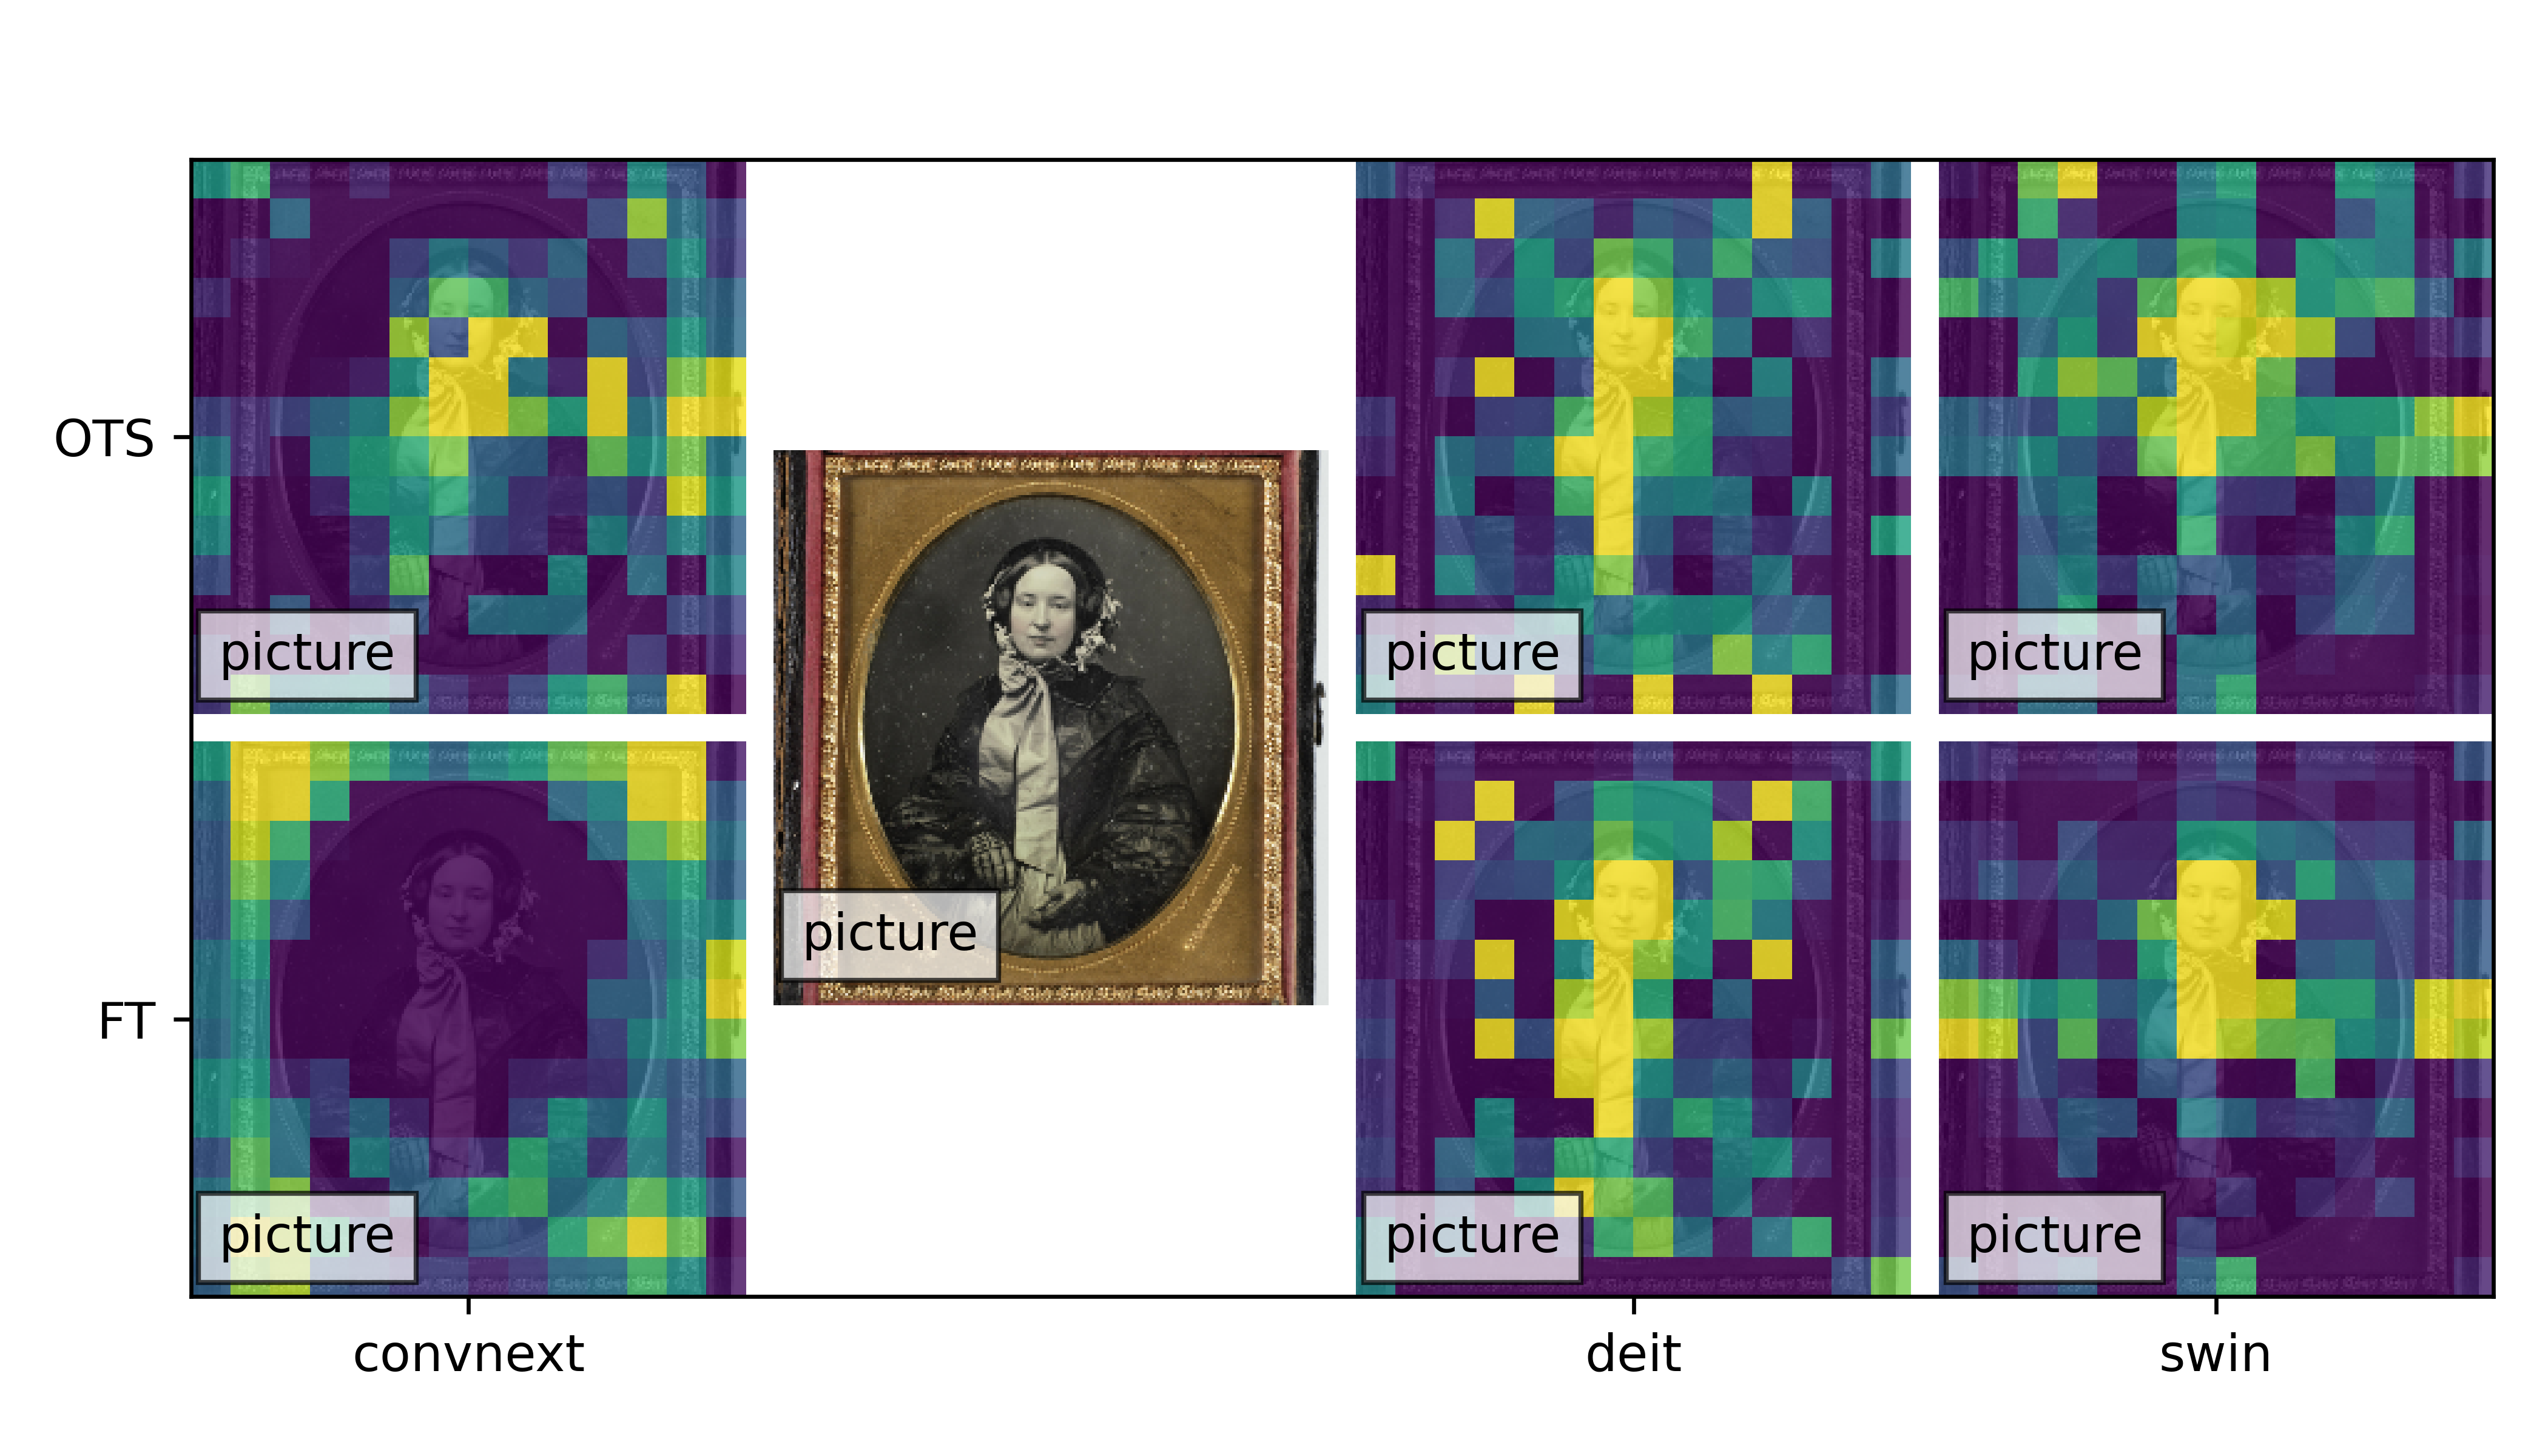
\includegraphics[width=8cm]{img/img011_salience.png}
    \caption{Picture}
    \label{results:img:sal:picture}
    \end{subfigure}
    \begin{subfigure}{0.49\textwidth}
    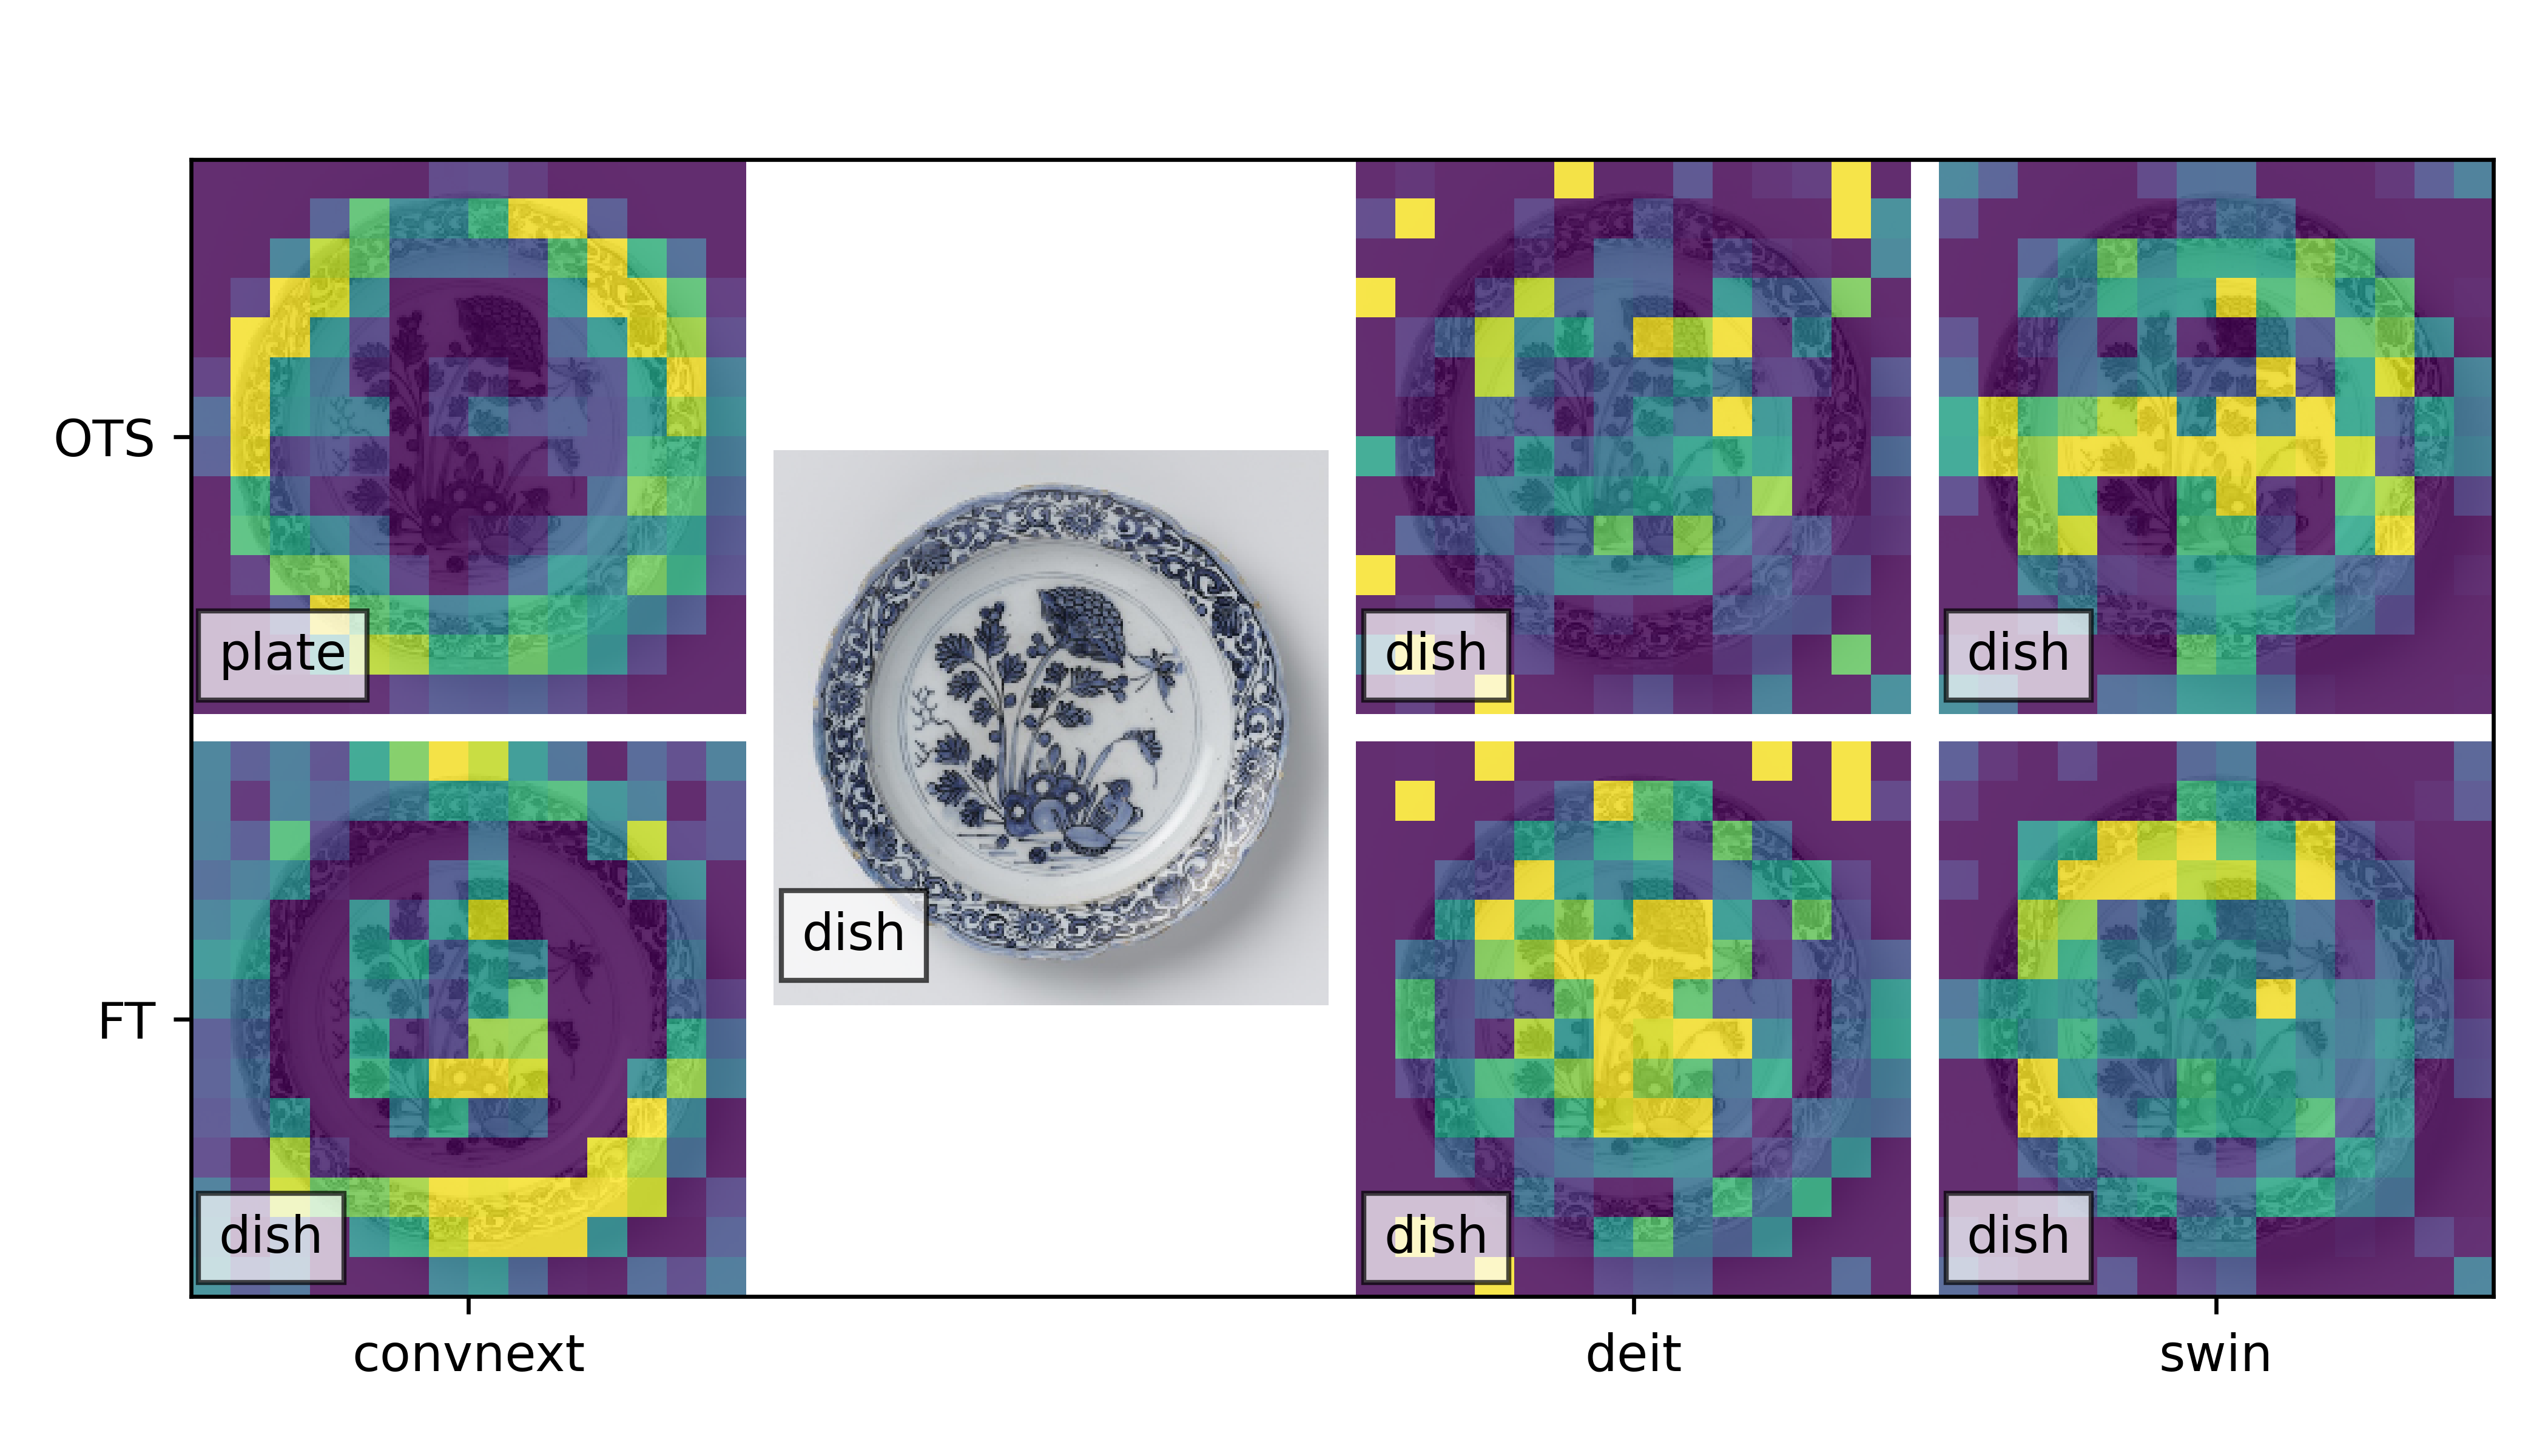
\includegraphics[width=8cm]{img/img005_salience.png}
    \caption{Dish}
    \label{results:img:sal:dish}
    \end{subfigure}
    \caption{Saliency maps for \texttt{ConvNext}, \texttt{DeiT}, and \texttt{Swin} after both off-the-shelf learning (OTS), and fine-tuning (FT). \texttt{ConvNext} appears to benefit more when training the whole model instead of the last layer, because it shows the biggest differences between OTS learning and FT. In the case of Figure \ref{results:img:sal:dish}, this even makes the difference between correct and incorrect classification.}
    \label{results:img:sal}
\end{figure*}

VTs and CNNs are much closer together after FT in Table \ref{results:tab:ft} than after OTS learning in Table \ref{results:tab:ots}. It is as if OTS learning already unlocks much of VTs' potential, while CNNs need an FT learning scheme for this.

Supporting `evidence' might be visible in Figure \ref{results:img:sal}. It plots saliency maps for one CNN (\texttt{ConvNext}), and two VTs (\texttt{DeiT} and \texttt{Swin}). It is interesting that \texttt{ConvNext} shows much bigger differences between the OTS and FT plots. In Figure \ref{results:img:sal:picture}, for example, it learns to just look at the picture frame after FT. In Figure \ref{results:img:sal:dish} it learns to look more at the center, which allows it to correctly classify the input as a dish instead of a plate\footnote{No idea what the difference is between these classes, but these models do seem to know, so that is good!}. % TODO Maybe delete this comment, not very professional
These bigger differences for \texttt{ConvNext} align well with observations made earlier, as they suggest that there is still much improvement possible after just OTS learning for CNNs.

The images in Figure \ref{results:img:sal} are representative examples, and show observations that could have been made from other images too. How representative the 3 models are for all 8 is debatable, and was not tested. In general, a big disclaimer should be added to these results, because some hand waving is involved. Importantly, 3 different salience mapping techniques were used: GradCam \citep{selvaraju2017grad} was implemented for \texttt{ConvNext}, while Attention Rollout \citep{abnar2020quantifying} was implemented for \texttt{DeiT}. This already makes the comparison somewhat unfair, and it becomes even worse when \texttt{Swin} is added, for which a self-invented method was used. This method is similar to GradCam, but instead of multiplying \textit{average} CNN channel gradients with said channel's activation, it directly multiplies activation with corresponding gradients in the output of one of the later transformer blocks\footnote{For the full implementation of all techniques, one is referred to the source code on: \\ \url{https://github.com/IndoorAdventurer/ViTTransferLearningForArtClassification}.}. Despite this, saliency maps were included, as they are interesting nonetheless.
% Show saliency maps here
% MENTION TECHNIQUES AND SHORTCOMMINGS!!!

\subsubsection{Overall}

\paragraph{Why does \textit{Artist classification} show the best overall performance?}
This might seem counter-intuitive: one would think that it is much easier to determine if something is a painting or a sculpture, than determining who the creator is. However, because only the top 30 classes are used, this is not necessarily true.

Figure \ref{methods:eg} shows example images for all tasks. On the one hand, it shows much heterogeneity for the \textit{Artist classification} task, with artists working in very different styles and mediums. On the other hand, it also shows difficulties for the other tasks: \textit{Material classification}, which seems to be the most challenging task, shows examples of both big differences within classes (note how the two instances of porcelain are very different), and small differences between classes (note how the porcelain plate is similar to the faience plate).

Then there is the problem of balance. It was mentioned earlier that balanced accuracy falls behind plain accuracy the most for \textit{Material classification}, and the least for \textit{Artist classification}. At the same time, Table \ref{methods:datasets} shows that it is also \textit{Material classification} which is the least balanced (Gini-coefficient of 0.563), while it is \textit{Artist classification} that is the most balanced (coefficient 0.236). This suggests that balance has a positive effect on testing accuracy, from which \textit{Artist classification}, in that case, benefits the most.

% Sabatelli different
% GINI COEFFICIENTS HYPOTHESIS!!!:
% This seems counterintuitive, as one would think artist identification is much more challenging than determining if something is a painting, or if it is made out of paper instead of wood. An explanation can likely be found in table \ref{methods:datasets}, which shows that material and artist classification sets are the least and most balanced, respectively. In addition, tables \ref{results:tab:ots_type} through \ref{results:tab:ots_artist} show that balanced accuracies are up to 14\% lower than plain ones for material classification, while they are much closer for artist classification. This suggests much accuracy is lost by misclassifying instances of less occurring classes in favor of more occurring ones. Similar finding can be done for FT results in section \ref{results:ft}.

\paragraph{The same hyperparameters are used for all models. Is this fair?}
The final learning scheme was chosen after extensive hyperparameter optimization, and was partially inspired by related work. It is possible that doing this for each model individually would have resulted in \textit{slightly} higher performances. This paper, however, does not aim to get the best possible performance, but instead wants to see how models compare to one another. It is unlikely that individually tuning each model would have changed overall findings.

A small asterisk to be made here, is that VTs might benefit more from better regularisation than CNNs (see section \ref{exp:int:ft}). Still, final accuracy should not be the only concern, because ease of use (i.e. effort needed to find the right hyperparameters) will also determine to what degree VTs are a valuable alternative to CNNs. Moreover, the main finding of this paper seems to be that VTs are able to perform on par with CNNs. Slightly better performance for VTs would not exactly hurt this finding.

% Preliminary studies
% Not about getting the best overall performance, but seeing how they compare to one another
% Asterix is that VTs might be able to do better, but then again -> Its also about ease of use

\paragraph{To what extent are the chosen models representative of all VTs and CNNs?}
Most models were selected because of their mention in related work. Notable exceptions are \texttt{ConvNext} and \texttt{EfficientNetV2}, which were selected because they are equally recent as the used VTs. Many of these models are popular/common, but one can't say that they are a representative sample. The question, of course, also is not how VTs and CNNs as a group compare to one another. Instead, the question is if the VT landscape as a whole has something to offer that could be an interesting alternative to common CNNs.

It is also interesting to wonder if, for example, `tiny'- or `medium'-sized version should have been used instead of `base' versions. All available `tiny' models were tested as well, and results have been reported where appropriate (e.g. section \ref{exp:int:ft}). Overall, however, these results did not suggest that using `tiny' versions would have made much of a difference for the rankings: `tiny' \texttt{Swin} and \texttt{ConvNext}, for example, remained superior under that circumstance.

\paragraph{What can be concluded from the results presented?}

\begin{figure}[tbh]
    \centering
    \def\svgwidth{7.7cm}
    \input{img/ots_vs_ft_type.pdf_tex}
    \caption{Time/accuracy trade-offs for VTs and CNNs either off-the-shelf or fine-tuned. Fine-tuned CNNs seem to make the best trade-off here, with one even appearing left above all off-the-shelf VTs. The best overall performance is achieved by a fine-tuned VT.}
    \label{results:img:ots_vs_ft_type}
\end{figure}

After OTS learning, results are slightly better for VTs, while after FT, results are almost the same for CNNs and VTs. With that said, it seems, VTs are very much able to perform on par with CNNs on the described art classification problems. Especially \texttt{Swin} and \texttt{DeiT} showed promising performance, and together with \texttt{ConvNext}, might be interesting models to consider.

Of course, final accuracy is not the full story, since time/accuracy trade-offs, for example, can also determine which model is preferred. Figure \ref{results:img:ots_vs_ft_type} plots the \textit{Type classification} accuracies of Tables \ref{results:tab:ots} and \ref{results:tab:ft} against training time per epoch. Total training time was not chosen instead, as this measure depends much more on selected hyperparameters.

The best overall performing model is a fine-tuned VT (\texttt{Swin}). At the same time, it is perhaps a CNN that shows the best time/accuracy trade-offs, because it performs better than any OTS-trained model, while still taking less time per epoch than any OTS-trained VT. The particular CNN this concerns, is \texttt{ResNet50}. Recall that this model only had 25.6 million parameters, while most VTs had around 86 million.

All `tiny' VTs are around the same size as \texttt{ResNet50}, and using these would have changed the situation completely. As such, taking Figure \ref{results:img:ots_vs_ft_type} with a grain of salt would be appropriate.

Still, it seemed fitting to conclude with this figure, as it neatly summarises all the main findings done in this section.
